\chapter{Анализ поставленной задачи}
\label{ch:analysis}

\section{Анализ требований к ПО}

\subsection{Формулировка требований в области проблем и в области решений}

\subsubsection{Требования в области проблем}

\begin{itemize}
    \item Супервизоры и руководители отдела должны иметь доступ к отчетам реального времени в PMS\@.
    \item Супервизоры и руководители отдела должны иметь возможность настраивать представление отчетов по своему усмотрению, в том числе изменять позицию и какие показатели нужно выводить.
    \item Пользователь с ролью «Аналитик» должен иметь возможность просматривать статистику пройденных испытаний в экранной форме или в печатной форме.
    \item RRS должен уметь обрабатывать большое количество данных в реальном времени, с опозданием на не более 1 секунду.
    \item Супервизоры и руководители отдела должны иметь возможность настраивать периодичность обновления отчетов, но не менее чем раз в 1 секунду.
    \item Администраторы PMS должны иметь возможность изменять период очистки данных из БД.
\end{itemize}

\subsubsection{Требования в области решений}

\Define{Redis}{резидентная система управления базами данных класса NoSQL с открытым исходным кодом, работающая со структурами данных типа <<ключ -- значение>>}
\Define{NauSnitch}{подсистема сбора данных по call-центру}
\begin{itemize}
    \item В качестве БД необходимо использовать СУБД PostgreSQL или Oracle DB для данных не чувствительных ко времени и СУБД Redis для чувствительных данных.
    \item Клиентской средой является PMS\@.
    \item Для разработки NauSnitch должны применяться технологии с высокой степенью параллелизма, масштабируемости и эффективной утилизацией ресурсов.
\end{itemize}

\subsection{Анализ требований}

\begin{itemize}
    \item Система должна давать возможность настройки отображения отчетов.
    \item Система должна очищать данные в БД через настраиваемый промежуток времени.
    \item Система должна успешно функционировать при одновременной работе 900 операторов.
    \item Максимальное время опоздания обновления состояния call-центра не должно превышать 1 секунду.
    \item Система должна справляться с нагрузкой в 2--3 события за 1 мс.
    \item Система должна потреблять не более 2Гб ОЗУ.
    \item Система должна эффективно работать на ЦП с более чем 24 ядрами.
\end{itemize}

\subsection{Обоснование архитектуры сервиса}

Общее описание архитектуры сервиса представлено на диаграмме~\ref{pic:archimate:summary}.

\begin{figure}[ht]
    \centering
    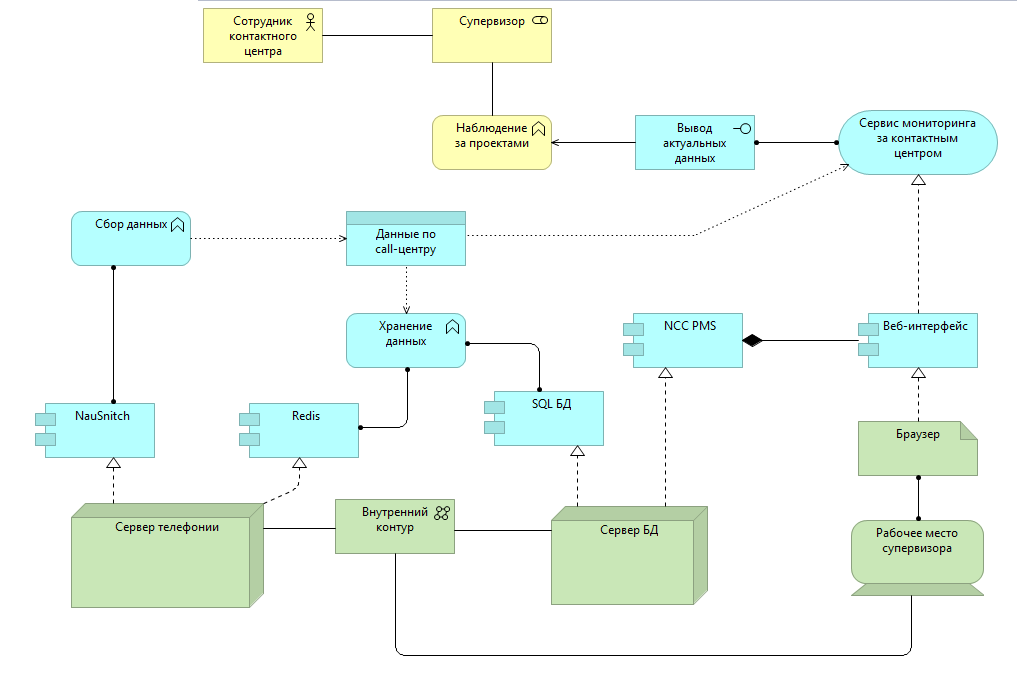
\includegraphics[width=\textwidth]{inc/img/archimate_summary}
    \caption{Архитектура проектируемой системы на Archimate}
    \label{pic:archimate:summary}
\end{figure}

Исходя из требований разрабатываемая архитектура
сервиса должна уметь выдерживать высокие нагрузки и уметь эффективно масштабироваться.

Основной задачей, с точки зрения архитектуры,
для RRS является преобразование сообщений, получаемых из шины в удобный для манипуляций формат,
сохранение их в общее хранилище и получение оттуда уже в удобном для отображения виде.
Другими словами такое поведение можно описать как реакцию на сообщения из NauCore,
т.~е. для такой системы подходящий вариант архитектуры является event-driven модель~\cite{software-architecture-patterns}.
Событийно ориентированная архитектура позволяет изолировано менять внутренее состояние сервиса как реакцию на
отдельные события, так же изоляция реакций позволяет писать простой асинхронный и легко масштабируемый код.
А используя принципы из реактивного манифеста~\cite{reactive-manifesto} можно добиться высокой отказоустойчивости и интерактивности сервиса.

Отделение подсистемы взаимодействия с пользователем от подсистемы сбора данных по call-центру,
позволит лучше контролировать нагрузку на сервис,
т.к. в нашем случае слабым звеном является подсистема сбора
и при высоких нагрузках достаточно увеличить количество запущенных экземпляров только этой подсистемы.
Так же, разделение этих двух подсистем на отдельные
исполняемые единицы позволит переиспользовать наработки с предыдущей попытке реализации RRS\@,
т.к. общение между ними происходит через публичное и фиксированные API\@.

\section{Выбор инструментальных средств}

Проанализировав собранные требования, подсистему взаимодействия с пользователем было решено
использовать оставшуюся с предыдущей версии сервиса для агрегирования информации по call-центру.
Предыдушая реализация была выполнена на базе PMS, она была написана как пакет на языке Java с
использованием фрэймворка Spring.
Такая реализация полностью удовлетворяет новым требованиям
и, благодаря взаимодействию с другими подсистемами только через публичный API,
не требует внесение каких-либо изменений или доработок для взаимодействие с новыми подсистемами.

Для подсистемы хранения чувствительной ко времени информарции будет использоваться
<<key -- value>> хранилище Redis.
Redis это высокооэффективное хранилище~\cite{HowfastisRedis},
которая хранит свои данные в оперативной памяти,
что обеспечивает высокую скорость доступа к ним.
Хранение данных в памяти помимо достоинств обладает еще одним недостатком --
в случае аварии данные будут утеряны,
но в нашем случае этот недостаток позволяет выполнить требование об очистки данных (см.~пункт~\S~\ref{subsubsec:требования-по-сохранности-информации-при-авариях}).
Таким образом Redis является отличным решением для использования как подсистему хранения
чувствительных ко времени данных.

Требования к подсистеме хранения нечувствительной ко времени информации сильно ограничивают
в выборе инструментальных средств, т.к. NCC гарантирует (см.~пункт~\S~\ref{subsubsec:требования-к-программному-обеспечению}),
что будет работать с такими БД, как PostgreSQL и Oracle,
ничего не остается, кроме как использовать их в качестве подсистемы.

К подсистеме сбора данных по call-центру предъявляются
высокие требования в плане производительности и масштабируемости.
Проанализировав предоставляемые на текущий момент инструментальные средства,
были выделены основные фавориты и среди них окончательно был выбран язык Go без использования
каких-либо фрэймворках.

Преимущества Go как платформы для реализации сервиса~\cite{the-pros-and-cons-of-programming-in-go}:
\begin{itemize}
    \item язык Go достаточно востребован~\cite{Наиболеевостребованныеязыкипрограммирования2018,ЗарплатыИТспециалистовнасередину2018года}
    и популярен~\cite{TIOBEIndex}
    на рынке, поэтому найти специалистов не составит труда;
    \item язык специально был спроектирован что бы быть простым и понятным~\cite{GoХорошийплохойзлой,ОплюсахиминусахGo,WhyGosdesignisadisservicetointelligentprogrammers};
    \item простая и эффективная модель реализации конкурентного и ассинхронного программирования~\cite{хоар1989взаимодействующие};
    \item в стандартной поставке присутствуют удобные и современные средства для диагностирования проблем производительности~\cite{ProfilingGoPrograms,ПрофилированиеиоптимизацияпрограммнаGo},
    утечек памяти и состояния гонок;
    \item в качестве артефакта сборки предоставляет самодостаточный исполняемый файл,
    статически скомпилированный со всеми необходимыми библиотеками,
    что сильно упрощает доставку и развертывание сервиса;
    \item решения, написанные на Go являются достаточно производительными и эффективными в потреблении аппаратных ресурсов~\cite{HowWeWentfrom30Serversto2Go,МиллионWebSocketиGo,ОпытпримененияGoвпродакшенеЯндекса};
    \item по сравнению с Python обладает статической типизацией, что облегчает выполнение рефакторинга и поддержку кодовой базы.
\end{itemize}

В тоже время есть и несколько недостатков~\cite{GoХорошийплохойзлой,50ShadesofGo}:
\begin{enumerate}
    \item типизация не достаточно строгая и не мешает совершать некоторые виды ошибок~\cite{СтатическийанализвGo};
    \item язык и его экосистема еще слишком не зрелая:
    \begin{enumerate}
        \item отсутствуют средства для контроля и версионирования сторонних библиотек;
        \item отсутствует стабильный драйвер для Oracle DB, есть только несколько, находящихся в экспериментальном режиме;
        \item отсутствуют библиотеки для простой работы с XML\@.
    \end{enumerate}
\end{enumerate}

Остальные расмотренные языки:
\begin{itemize}
    \item Python -- уже была неудачная попытка и отсутствует понимание куда дальше двигаться в этом направлении;
    \item C/C++ -- разработка на этих языках представляет из себя слишком долгий и дорогой процесс~\cite{ОпытпримененияGoвпродакшенеЯндекса};
    \item Rust -- пока еще слишком новый, сложный в изучении и достаточно тяжело найти необходимых специалистов;
    \item Java -- неэффективно расходует аппаратные ресурсы, в том числе оперативную память,
    сложно организовать асинхронные и неблокирующие операции;
    \item Node.js -- работает в одном потоке, отличий от Python в плане производительности почти нет.
\end{itemize}

\Define{NATS}{система обмена сообщениями с открытыми исходными кодами~\cite{AboutNATS}}
Шина обмена сообщений NauCore и используемый протокол NCC, NCC2 и NCCN является
внутренней проприетарной разработкой.
Этот факт сильно ограничивает выбор реализаций этого протокола,
на момент начала разработки были доступны реализации на языках программирования: C, Java и Python.
Таким образом, требовалось написать новую реализацию протокола на Go.
При этом она должна удовлетворять требованиям по производительности
и уметь работать с сообщениями асинхронно.
Такая реализация требовала большого количества времени и сил,
поэтому было решено сделать шлюз между NauCore и
уже существующей популярной высокопроизводительной open-source шиной,
к которой есть реализация клиента на языка Go.
И такой шиной является NATS, к тому же она сама написана на языке Go,
что, в дальнейшем, позволило интегрировать ее в NauSnitch.

\section{Функциональная модель}

Описание функциональной модели выполнено в нотации IDEF0 на рисунке~\ref{pic:idef0:a0}.
В качестве объекта описания с помощью функциональной модели была выбрана основная функция RRS --
мониторинг за текущим состоянием call-центра и оперативное реагирование на изменения состояния.

На рисунке~\ref{pic:idef0:a0:decompose} показана декомпозиция диаграммы вернего уровня,
а на рисунках~\ref{pic:idef0:a1:decompose}~и~\ref{pic:idef0:a2:decompose} декомпозиция функциональных блоков.

\begin{figure}[ht]
    \centering
    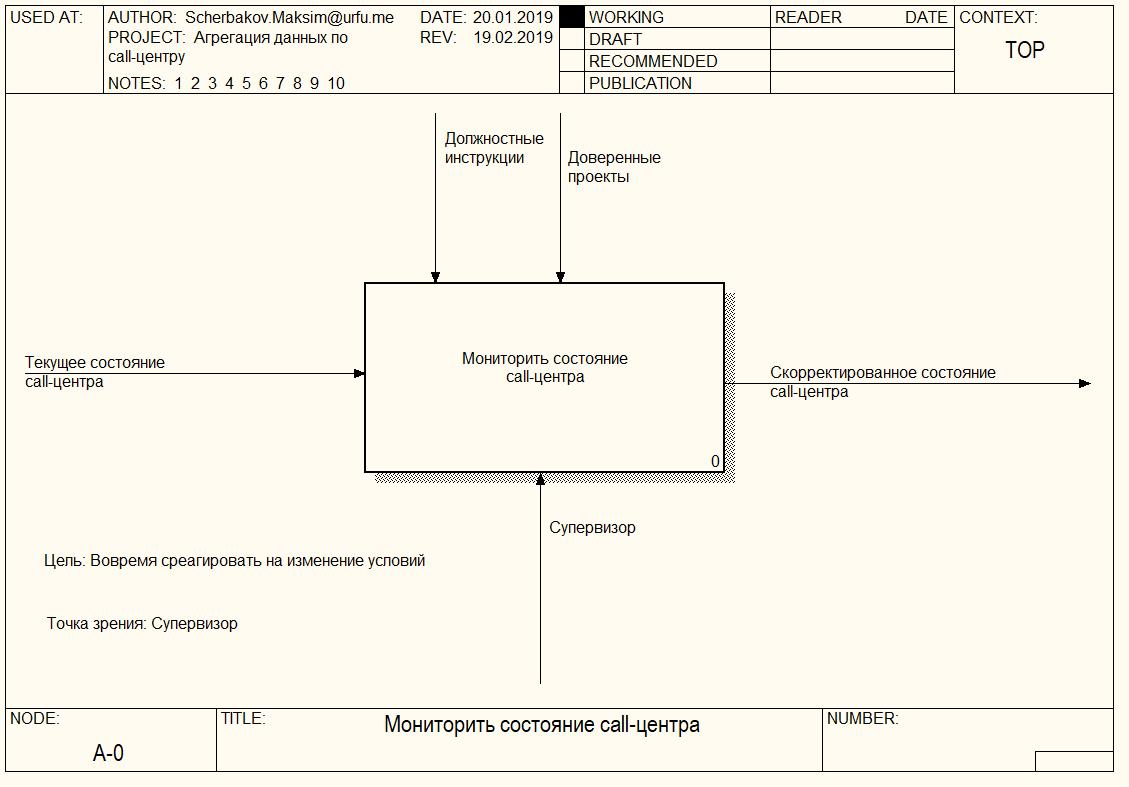
\includegraphics[width=\textwidth]{inc/img/diagram0}
    \caption{Функциональная модель мониторинга состояния call-центра в IDEF0}
    \label{pic:idef0:a0}
\end{figure}

\begin{figure}[ht]
    \centering
    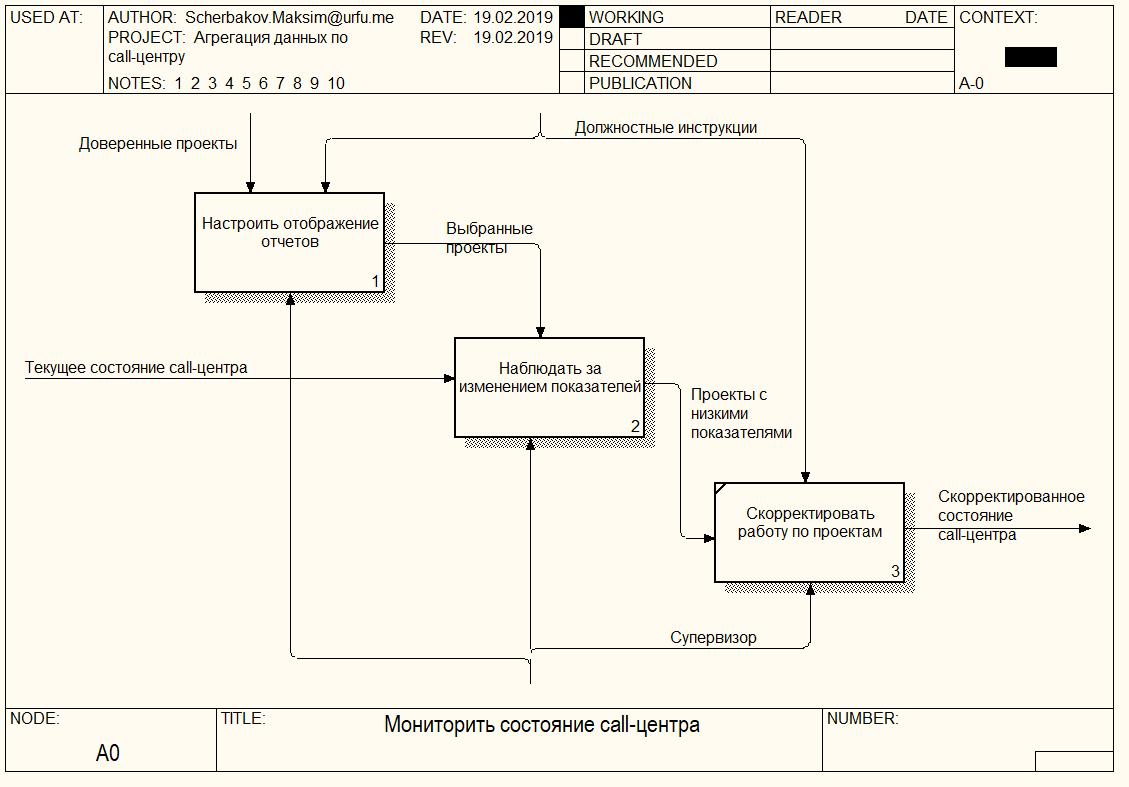
\includegraphics[width=\textwidth]{inc/img/diagram1}
    \caption{Декомпозиция функциональной модели А-0}
    \label{pic:idef0:a0:decompose}
\end{figure}

\begin{figure}[ht]
    \centering
    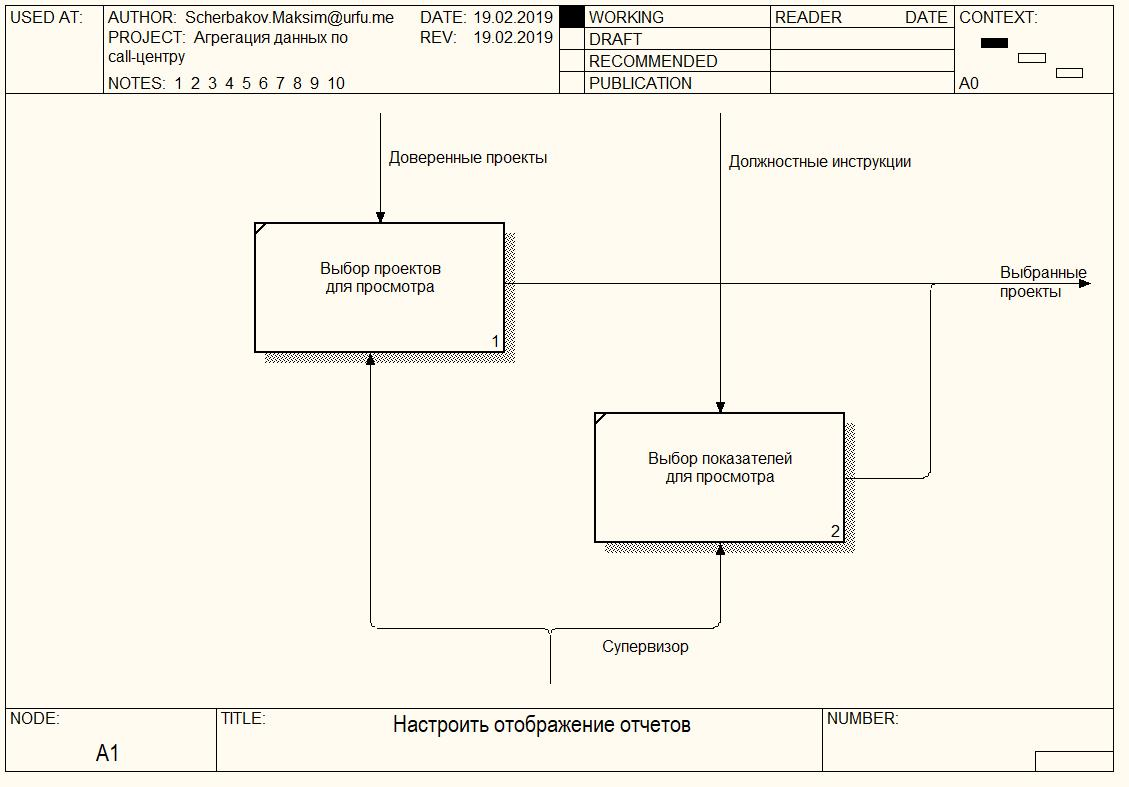
\includegraphics[width=\textwidth]{inc/img/diagram2}
    \caption{Декомпозиция блока <<Настроить отображения отчетов>>}
    \label{pic:idef0:a1:decompose}
\end{figure}

\begin{figure}[ht]
    \centering
    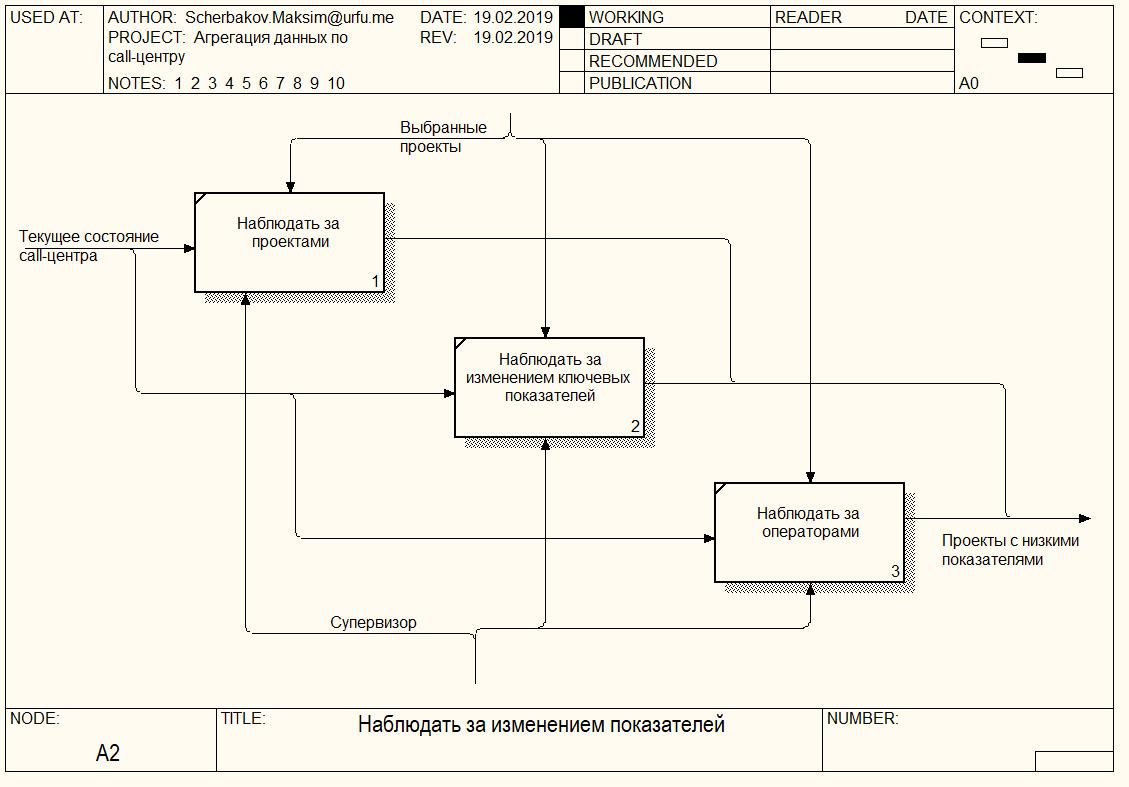
\includegraphics[width=\textwidth]{inc/img/diagram4}
    \caption{Декомпозиция блока <<Наблюдать за изменениями показателей>>}
    \label{pic:idef0:a2:decompose}
\end{figure}

\section{Обоснование интерфейса пользователя}

Обоснование интерфейса пользователя будем проводить методом А.~Купера~\cite{cooper2014face}.

\subsection{Разработка и описание персонажа}

\subsubsection{Ключевой персонаж}

Образ персонажа изображен на рисунке~\ref{pic:pcharacter}.

\begin{figure}
    \centering
    % [width=0.5\textwidth] --- регулировка ширины картинки
    
\includegraphics[width=0.5\textwidth]{inc/img/pchar}
    \caption{Ключевой персонаж}
    \label{pic:pcharacter}
\end{figure}

\noindent Имя: Валерий. \\
Возраст: 26. \\
Образование: высшее. \\
Супервизор в тех. поддержке ПО. \\
Женат, детей пока нет.

Компьютер использует на работе,
в личное время предпочитает использовать более мобильные гаджеты,
такие как смартфон, планшет, иногда использует личный ноутбук,
но в основном по рабочим целям.
В коллективе ценит прогрессивный настрой, стремление развиваться.

\subsubsection{Цели}

Бизнес-цели:
\begin{itemize}
    \item вовремя реагировать на нештатные ситуации;
    \item полностью контролировать текущую обстановку по доверенным проектам, чтобы иметь возможность оптимизировать нагрузку и увеличивать различные KPI\@.
\end{itemize}

Персональные цели: получить повышение.

\subsection{Описание персонажа и его требований}

\subsubsection{Сценарии}

Ежедневные сценарии работы:
\begin{itemize}
    \item ежедневный аудит подконтрольных проектов;
    \item наблюдение за недобросовестными операторами.
\end{itemize}

Эпизодические сценарии работы:
\begin{itemize}
    \item вышла новая версия ПО, резко подскочило количество вызовов в тех. поддержку, на проекте не хватает операторов, нужно перераспределить из менее загруженных проектов;
    \item по проекту постепенно начали снижаться ключевые показатели, нужно разобраться в чем дело.
\end{itemize}

Типичный день.

Валерий едет утром на работу, ему нужно успеть приехать чуть пораньше остальных,
последнее время он заметил, что Константин (оператор, стажер)
стал халатно относиться к своей работе,
и Валерию нужно настроить рабочее место Константина,
чтобы подтвердить или опровергнуть свою теорию.
Когда Валерий пришел в офис, там почти никого не было,
только вяло собирались пара операторов с ночной смены
и на Валерия они не обращали никакого внимания,
он быстро сделал свои дела и пошел в буфет, выпить чашечку кофе.

К восьми в офис начали подтягиваться первые работники, обстановка оживилась,
но супервизор уже приступил к своей работе,
ему еще предстояло проверить состояние проектов за эту ночь,
прослушать пару записей, благо ночью их было не много,
и выставить оценку работы операторов.
До обеда Валерий успел проверить ночные звонки и принять участие в
видеоконференции - один из операторов попросил помощи,
т.~к. у него возникли сложности с вопросом от клиента.

На обед Валерий пошел со своими друзьями-супервизорами, они обсуждали нового стажера оператора: думали, как его можно было бы замотивировать к работе. Возвращаясь с обеда Валерий заскочил в комнату отдыха, где развалился на удобном пуфике и на своем ноутбуке (который он всегда берет с собой) начал просматривать различные новости в интернете, в фоне у него была открыта вкладка с таблицей ключевых показателей, в которой фигурировал оператор Константин.

Примерно через час эту идиллию прервал звонок от руководителя отдела, он напомнил Валерию, что в пол третьего им нужно собраться, чтобы решить проблему резких нагрузок на определенные проекты, один из таких проектов был на попечительстве у Валерия. Так как у него оставалось еще где-то пол часа, Валерий пошел на свое рабочее место, попутно решив пару вопросов, которые задавали операторы, увидев, как он проходит мимо. На рабочем месте он оценил текущее состояние доверенных ему проектов, добавил пару задач, кое-где немного изменил настройки, в общем, занимался обычной рутиной. Чуть позже на совещании руководители решили создать резерв из операторов с низкой нагрузкой для того, чтобы их в любое время можно было распределить на критические проекты, от Валерия требовалось создать нужный проект и выделить туда пару своих операторов.

Под конец рабочего дня Валерию оставалось только заняться прослушиванием и оценкой сделанных за день звонков, это занимало не мало времени, поэтому он всегда оставлял такую работу в конце.

Уже по дороге домой в метро Валерий вспомнил, что забыл посмотреть какие были результаты работы за день у Константина, он достал свой ноутбук начал изучать показатели стажера, к несчастью, его мысли подтвердились и Костя действительно пол дня пробыл в статусе «не беспокоить», что бы на него не распределялись вызовы. Видимо завтра с ним предстоит серьезный разговор.

\subsubsection{Требования персонажа к ПО, важность требований и частота функциональности}

Программа должна:
\begin{itemize}
    \item предоставлять возможность просматривать график изменений ключевых показателей по проекту;
    \item давать возможность просматривать текущее состояние выбранных проектов;
    \item обновлять показатели с заданной периодичностью;
    \item иметь наглядную сводку по входящим проектам;
    \item давать возможность с помощью модуля можно просматривать текущее состояние выбранных операторов;
    \item иметь не перегруженный интерфейс, чтобы в программе можно было легко сориентироваться;
    \item давать возможность указать, какие данные выводить в отчет;
\end{itemize}

\subsubsection{Важность пользовательских требований}

Следующие значения важности использованы в таблице~\ref{tab:req:importance}:
\begin{itemize}
    \item $+2$ --- персонаж испытывает необходимость в данной возможности;
    \item $+1$ --- персонаж не отказался бы от такой возможности;
    \item $0$ --- персонажу не мешает данное требование;
    \item $-1$ --- персонажу мешает данное требование;
    \item $-2$ --- данное требование значительно затрудняет работу персонажа.
\end{itemize}

\begin{table}[ht]
    \caption{Требования по важности}
    \begin{small}
        \begin{tabular}{|p{0.7\textwidth}|p{0.2\textwidth}|}
            \hline
            Требование                          & Оценка \\
            \hline
            Возможность просматривать график ключевых показателей по проекту & $+2$  \\
            \hline
            Просмотр текущего состояния выбранных проектов           & $+2$    \\
            \hline
            Обновление показателей с заданной периодичностью               & $-1$ \\
            \hline
            Не перегруженный интерфейс               & $0$ \\
            \hline
            Наглядная сводка по входящим проектам               & $+1$ \\
            \hline
            Отображение текущего состояния выбранных операторов & $+2$ \\
            \hline
            Настройка, какие данные нужно отображать в отчете               & $+2$ \\
            \hline
        \end{tabular}
    \end{small}
    \label{tab:req:importance}
\end{table}

\subsubsection{Частота использования функций}

Следующие значения частот использованы в таблице~\ref{tab:req:frequency}:
\begin{itemize}
    \item $2$ --- используется персонажем несколько раз в неделю;
    \item $1$ --- используется персонажем 1-2 раз в месяц;
    \item $0$ --- используется персонажем 1-2 раза в год или не используется вообще.
\end{itemize}

\begin{table}[ht]
    \caption{Требования по частоте}
    \begin{small}
        \begin{tabular}{|p{0.7\textwidth}|p{0.2\textwidth}|}
            \hline
            Требование                          & Оценка \\
            \hline
            Возможность просматривать график ключевых показателей по проекту & $2$  \\
            \hline
            Просмотр текущего состояния выбранных проектов          & $2$    \\
            \hline
            Наглядная сводка по входящим проектам               & $2$ \\
            \hline
            Отображение текущего состояния выбранных операторов              & $2$ \\
            \hline
            Настройка, какие данные нужно отображать в отчете              & $1$ \\
            \hline
        \end{tabular}
    \end{small}
    \label{tab:req:frequency}
\end{table}

\subsection{Информационная структура разрабатываемой системы}
\label{subsec:информационная-структура-разрабатываемой-системы}

На основе требований к проектируемому ПО можно предложить следующую информационную структуру:
\begin{itemize}
    \item сводка по выбранным входящим проектам;
    \item отчет по выбранным входящим проектам;
    \item отчет по выбранным исходящим проектам;
    \item информация о текущем состоянии выбранных операторов;
    \item график изменений ключевых показателей по текущему проекту.
\end{itemize}

Так как подсистема взаимодействия с пользователем (см.~пункт~\S~\ref{subsubsec:подсистема-взаимодействия-с-пользователем})
будет интегрирована в уже существующую систему,
нужно органично и не противоречиво разместить новые формы в уже существующей экосистеме.
Поэтому такие формы, как сводки по входящим проектам,
отчеты по входящим и исходящим
и информацию о текущем состоянии выбранных операторов имеет смысл разместить на существующей вкладке
«Отчет» в корне системы,
т.~к. эти отчеты не привязаны к конкретным операторам либо проектам и могут
отображать сразу несколько выбранных элементов.
А вот график изменения ключевых
показателей выводится по конкретному проекту и что бы пользователям было легче
ориентироваться разместим его только на форме проекта,
при этом выводимый график будет напрямую зависеть того,
какой проект выбран в данный момент.

\subsection{Реализация требований пользователя к разрабатываемой системе}

\subsubsection{Общая схема пользовательского интерфейса}

Подсистема взаимодействия с пользователем (см.~пункт~\S~\ref{subsubsec:подсистема-взаимодействия-с-пользователем})
будет представлять собой модуль для PMS\@.
Модуль добавляет несколько вкладок для отображения и настройки различных
типов отчетов реального времени.

Задача навигации по вкладкам остается на существующей системе,
нашей задачей будет разместить информацию на уже существующих формах для бесшовной интеграции.

Настройка информации для отображения осуществляется меню, предоставляемой PMS\@.

\subsubsection{Реализация отдельных пользовательских требований в интерфейсе}

Возможность просмотра изменения ключевых показателей по проекту.
Это требование будет реализовано временным графиком, расположенным на странице проекта, его можно увидеть на рисунке~\ref{pic:intr:proj:keyval}.

\begin{figure}[ht]
    \centering
    % [width=0.5\textwidth] --- регулировка ширины картинки
    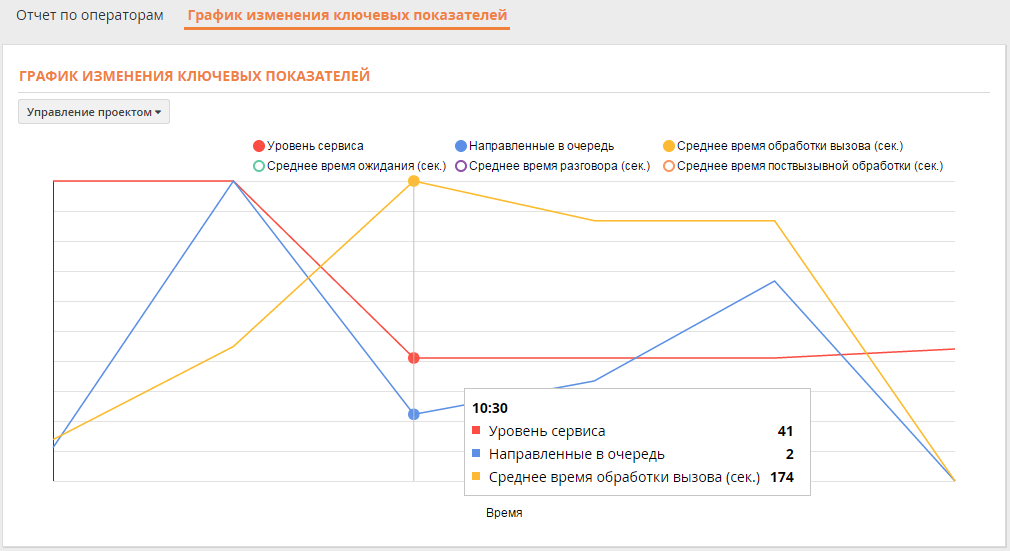
\includegraphics[width=0.85\textwidth]{inc/img/intr_key_chart}
    \caption{График изменения ключевых показателей в проекте}
    \label{pic:intr:proj:keyval}
\end{figure}

Просмотр текущего состояния выбранных проектов.
Для реализации этого требования будет сделано две сводные таблицы (рисунок~\ref{pic:intr:proj:incoming}~и~\ref{pic:intr:proj:outcoming}),
где строками будут выбранные проекты, а столбцами выбранная информация для них.
Для выбора проектов будет реализована специальная кнопка «Выбрать проекты»
\Define{Drag’n’Drop}{означает буквально тащи-и-бросай -- способ оперирования элементами интерфейса в интерфейсах пользователя (как графическим, так и текстовым, где элементы GUI реализованы при помощи псевдографики) при помощи манипулятора «мышь» или сенсорного экрана~\cite{Drag-and-drop}}
по нажатию на которую откроется Drag’n’Drop
меню с возможностью
выбрать активные проекты для отображения,
чтобы их выбрать достаточно перенести на панель справа.
Так же в меню будут доступны два переключателя:
«Отображать все» и «Скрыть блокированные».
Если выбрать «Отображать все», то в таблицу будут выведены все проекты,
в которых участвует супервизор.
При выборе «Скрыть блокированные» будут показаны только активные проекты (рисунок~\ref{pic:intr:proj:select}).

\begin{figure}[ht]
    \centering
    % [width=0.5\textwidth] --- регулировка ширины картинки
    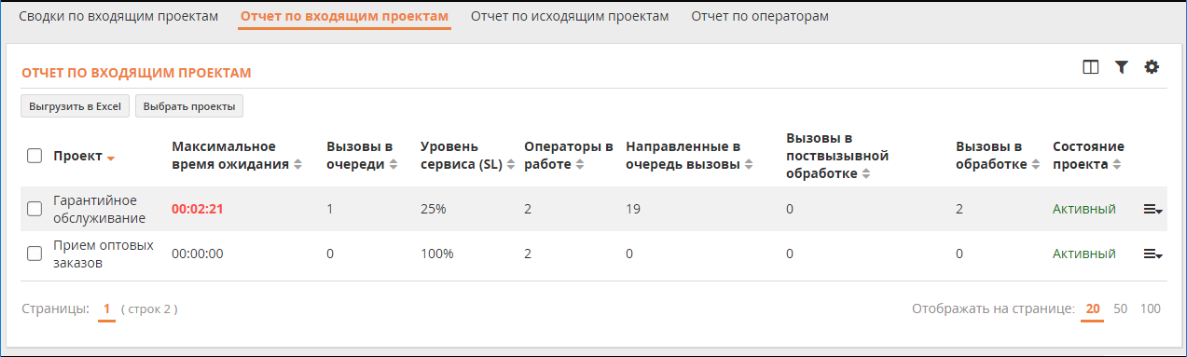
\includegraphics[width=0.85\textwidth]{inc/img/intr_incoming_proj}
    \caption{Отчет по входящим проектам}
    \label{pic:intr:proj:incoming}
\end{figure}

\begin{figure}[ht]
    \centering
    % [width=0.5\textwidth] --- регулировка ширины картинки
    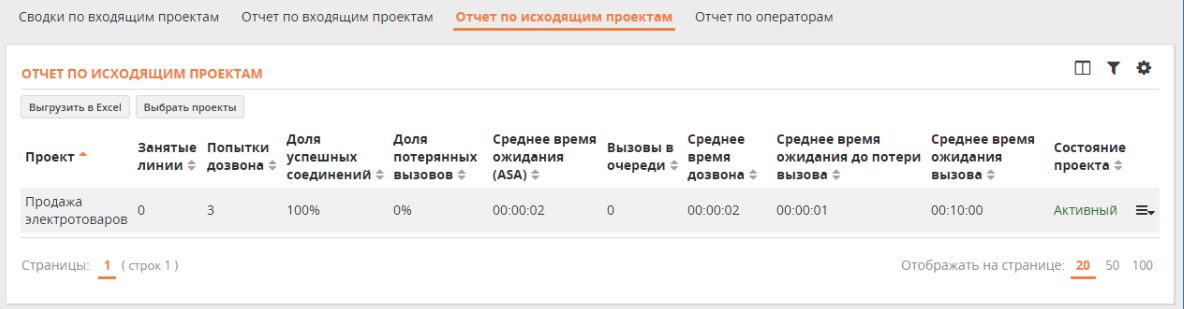
\includegraphics[width=0.85\textwidth]{inc/img/intr_outcoming_proj}
    \caption{Отчет по исходящим проектам}
    \label{pic:intr:proj:outcoming}
\end{figure}

\begin{figure}[ht]
    \centering
    % [width=0.5\textwidth] --- регулировка ширины картинки
    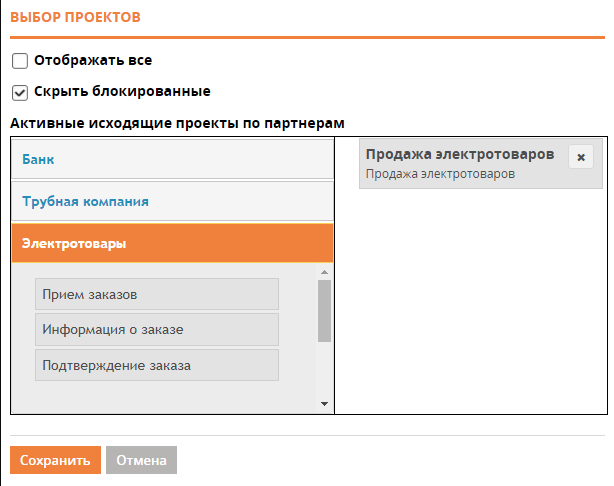
\includegraphics[width=0.5\textwidth]{inc/img/intr_select_proj}
    \caption{Форма выбора проектов для отображения}
    \label{pic:intr:proj:select}
\end{figure}

Наглядная сводка по входящим проектам.
Для наглядности в качестве формы отображения информации был выбран временной
график и краткая сводка,
все это было объединено в одной компактной форме,
что бы была возможность одновременно наблюдать сразу за несколькими проектами
(рисунок~\ref{pic:intr:proj:incoming:total}).

\begin{figure}[ht]
    \centering
    % [width=0.5\textwidth] --- регулировка ширины картинки
    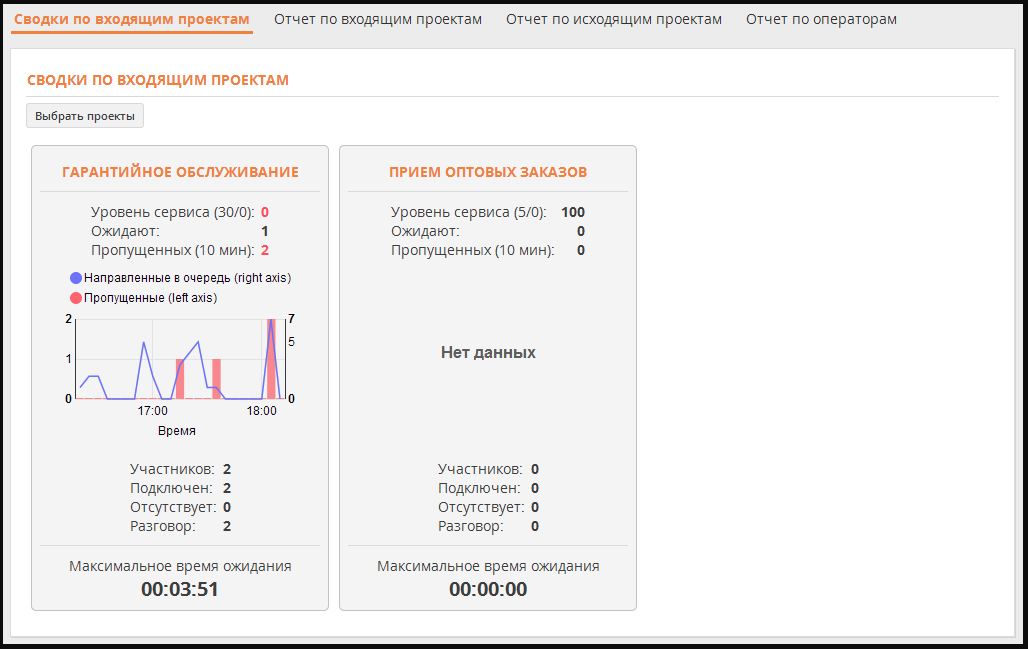
\includegraphics[width=0.85\textwidth]{inc/img/intr_incoming_proj_ttl}
    \caption{Сводка по входящим проектам}
    \label{pic:intr:proj:incoming:total}
\end{figure}

Отображение текущего состояния выбранных операторов.
Так как в принципе формат отображение и требования похожи
на требование по отображению текущего состояния выбранных проектов,
было решено сделать отображение текущего состояния операторов по такому
же принципу (рисунок~\ref{pic:intr:operator}).

\begin{figure}[ht]
    \centering
    % [width=0.5\textwidth] --- регулировка ширины картинки
    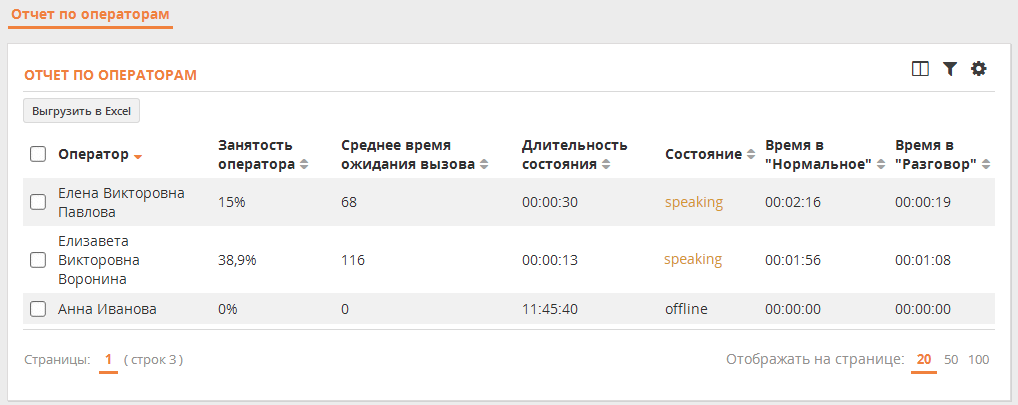
\includegraphics[width=0.85\textwidth]{inc/img/intr_operator}
    \caption{Отчет по операторам}
    \label{pic:intr:operator}
\end{figure}

Настройка, какие данные нужно отображать в отчете.
Настройка, каких конкретно проектов и операторов нужно отображать
была описана выше (рисунок~\ref{pic:intr:proj:select}).
Для настройки отображения только нужных показателей воспользуемся возможностями,
предоставляемыми системой,
а именно меню настройки отображения таблиц (рисунок~\ref{pic:intr:cfg:visible}),
нам остается только добавить нужные значения.

\begin{figure}[ht]
    \centering
    % [width=0.5\textwidth] --- регулировка ширины картинки
    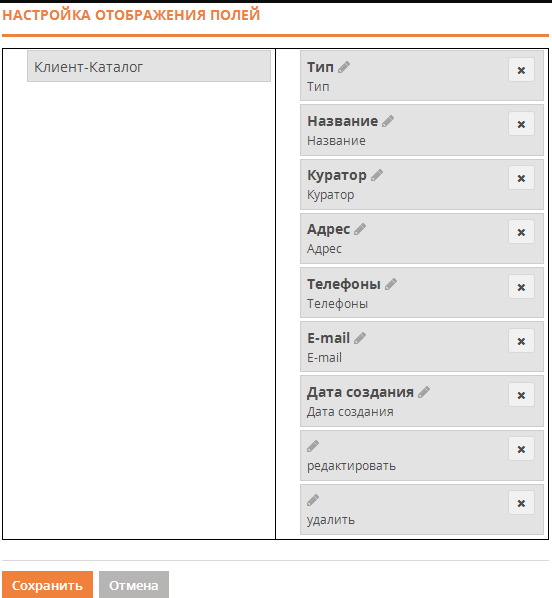
\includegraphics[width=0.6\textwidth]{inc/img/intr_cfg_visible}
    \caption{Форма настройки отображаемых полей}
    \label{pic:intr:cfg:visible}
\end{figure}